% subdivisões disponíveis: \chapter, \section, \artigo, \paragrafo, \paragrafounico, \inciso, \inciso\ itens

\documentclass[capitulo]{br-lex-2017}
\usepackage{graphicx}

\newcounter{anexonumero}

\newcommand{\anexo}[1]{\hfill Anexo \stepcounter{anexonumero}\theanexonumero: #1}

\begin{document}

\titulo{Lei Estadual Nº xxxx,\\de 18 de dezembro de 2019}
\descricao{Dispõe sobre a reorganização da Região Metropolitana de Curitiba (RMC) e dá outras providências}

\chapter{Da regionalização}

\artigo A nova regionalização da RMC conforme delimitado no anexo I deste desta Lei Complementar será dividida em:

\inciso Núcleo Urbano Consolidado;
\inciso Sub-região Norte;
\inciso Sub-região Sul;

\chapter{Da gestão}

\artigo A Coordenação da Região Metropolitana de Curitiba (COMEC) é Autarquia responsável pela administração e gestão do território metropolitano.

\artigo Criação do Departamento de Planejamento, voltado para as questões metropolitanas, composto por técnicos, irão nortear o desenvolvimento urbano e regional sustentável da Região Metropolitana de Curitiba (RMC).

	\paragrafo Os trabalhos do Departamento de Planejamento serão desenvolvidos de forma permanente e interfederativa e  deverão embasar permanentemente os ajustes às metas, projetos e ações que o Conselho Deliberativo vier a tomar.
	
	\paragrafo O Departamento de Planejamento poderá receber contribuição da comunidade técnico-científica para auxílio na análise e interpretação das informações, bem como na criação de indicadores específicos para o acompanhamento das ações de planejamento regional, na Região Metropolitana de Curitiba (RMC).
	
	\paragrafo O Departamento de Planejamento é composto por dimensões estruturantes e eixos integradores:
	
		\inciso as funções públicas de interesse comum da Região Metropolitana de Curitiba (RMC) que poderão ser aplicadas entre os municípios;
		
		\inciso o planejamento e a articulação dos municípios integrantes a respeito da mobilidade metropolitana;
		
		\inciso à articulação dos municípios no parcelamento, uso e ocupação do solo urbano;
		
		\inciso a delimitação das áreas com restrições à urbanização visando à proteção do patrimônio ambiental;
		
		\artigo Institui o Fundo de Investimento da Região Metropolitana de Curitiba (RMC), com gerência feito pela Coordenação da Região Metropolitana de Curitiba (COMEC).

\artigo Constituem receitas do Fundos de Desenvolvimento:

	\inciso recursos de natureza orçamentária que lhe forem destinados pela União, pelo Estado e pelos municípios situados em cada Região Metropolitana;
	
	\inciso produtos de operações de crédito realizadas pela União, Estado e Municípios situados nas Regiões Metropolitanas, destinados ao financiamento de atividade e projetos integrantes de programas de interesse metropolitano;
	
	\inciso retorno financeiro de empréstimo e subempréstimo para investimentos em obras e serviços no âmbito metropolitano;
	
	\inciso rendas auferidas com aplicação de seus recursos no mercado financeiro;
	
	\inciso recursos provenientes de taxas e contribuições de melhoria, arrecadadas pelo Estado ou pelos Municípios, relativas a empreendimentos e serviços de interesse metropolitano;
	
	\inciso transferências a fundo perdido, proveniente de entidades públicas ou privadas, nacionais, estrangeiras ou internacionais;
	
	\inciso recursos provenientes de outras fontes.

\artigo O Presidente dos Conselhos, Deliberativo e Consultivo não será mais feita por indicação direta do Governador do Estado.

\artigo A Diretoria de Transporte da Região Metropolitana de Curitiba (RMC) passa a ser subordinada do Conselho Deliberativo.

\artigo O Presidente do Conselho Deliberativo Consultivo deverão ser escolhido através de votação de todos os participantes da RMC com participação da sociedade civil e paridade em todos os votos.

\artigo Deverá ser garantida, no mínimo, a participação dos seguintes representantes no Conselho Deliberativo:

	\inciso representantes dos consórcios intermunicipais;
	
	\inciso representantes das secretarias de Estado vinculadas às funções públicas de interesse comum;
	
	\inciso representantes da sociedade civil e de entidades organizadas cujas áreas de atuação estejam relacionadas com as Funções Públicas de Interesse Comum (FPICs);
	
	\inciso representantes de órgãos federais cujas áreas de atuação estejam relacionadas com as Funções Públicas de Interesse Comum (FPICs);
	
	\inciso representantes do Departamento de Planejamento;
	
	\inciso representantes do Conselho Consultivo;

\artigo Deverá ser garantida, no mínimo, a participação dos seguintes representantes no Conselho Consultivo:

	\inciso representantes das secretarias de Estado vinculadas às funções públicas de interesse comum;
	
	\inciso representantes da sociedade civil e de entidades organizadas cujas áreas de atuação estejam relacionadas com as Funções Públicas de Interesse Comum (FPICs);
	
	\inciso representantes de órgãos federais cujas áreas de atuação estejam relacionadas com as Funções Públicas de Interesse Comum (FPICs);
	
	\inciso representantes do Departamento de Planejamento.

\artigo Os representantes do Estado do Paraná, dos Municípios integrantes da RMC e da sociedade civil, agentes da Governança Interfederativa da Região Metropolitana de Curitiba (RMC), deverão compartilhar esforços e ações para compatibilizar ações que visam a melhora na infraestrutura metropolitana.

\artigo O estabelecimento das Áreas de Intervenção Metropolitana e seus respectivos Planos de Ação Interfederativa devem ser precedidos por análise e discussão nos Conselhos e  submetidos ao acompanhamento do Departamento de Planejamento.

\chapter{Dos mecanismos de proteção ambiental}

\artigo Entendendo-se a importância de conter a expansão urbana para as franjas da Região Metropolitana de Curitiba (RMC), onde há a presença de mananciais. Para isso, pretende-se a criação de um cinturão verde em um raio de 15 km em volta do Núcleo Urbano Central.

	\paragrafounico São objetivos do Cinturão Verde:
	
		\inciso abrigar os mananciais que abastecem a Região Metropolitana;
		
		\inciso abrigar a biodiversidade;
		
		\inciso proteger os solos;
		
		\inciso conter as expansões irregulares em áreas de proteção;
		
		\inciso garantir a manutenção das áreas rurais com sua vocação atual;
		
		\inciso estimular atividades sustentáveis.

\artigo Estabelece-se a utilização de instrumentos garantidores da qualidade ambiental e asseguradores da vocação das franjas e de sua manutenção, a serem disciplinados por Lei Complementar:

\inciso Transferência do Direito de Construir (TDC);

\inciso ICMS Ecológico;

\inciso Pagamento por Serviços Ambientais (PSA).

\chapter{Dos mecanismos de colaboração e gestão interfederativa}

\artigo Os consórcios têm como objetivo a reunião dos municípios da Região Metropolitana de Curitiba (RMC) para planejamento, articulação e estabelecimento de agenda de caráter regional.

\paragrafo Os consórcios adotarão a forma de um Consórcio Público sob forma de associação pública.

\paragrafo Os consórcios adotarão o seguinte paradigma funcional:

\inciso cada município participante é membro da Secretaria Executiva;

\inciso um presidente e vice-presidente que são escolhidos anualmente por meio de votação dos demais prefeitos, tendo um mandato de dois anos;

\inciso haverá um Diretor Executivo, eleito por votação dos demais prefeitos, com o mesmo tempo de mandato.

\chapter{Das Funções Públicas de Uso Comum}

\artigo Estabelece o Sistema de Mobilidade e Transporte.

\paragrafo Os Sistemas Viário e de Transporte deverão promover a mobilidade de pessoas e mercadorias e a ordenação da ocupação do território, num padrão compatível com o desenvolvimento social e econômico.

\paragrafo Os Conselhos Deliberativo e Consultivo deverão promover a articulação, a discussão e o Departamento de Planejamento dar o suporte técnico para a implementação das ações inerentes, integrando-as às demais funções públicas de interesse comum e em interação com os municípios participantes da Região Metropolitana de Curitiba (RMC) uma vez que a eficiência dos sistemas Viário e de Transporte corresponde à eficiência social e econômica do espaço que neles se materializa, cuja defesa tem caráter permanente.

\chapter*{Anexos}

	\begin{figure}[h!]
		\centering
		\anexo{Nova regionalização da Região Metropolitana de Curitiba (RMC)}
		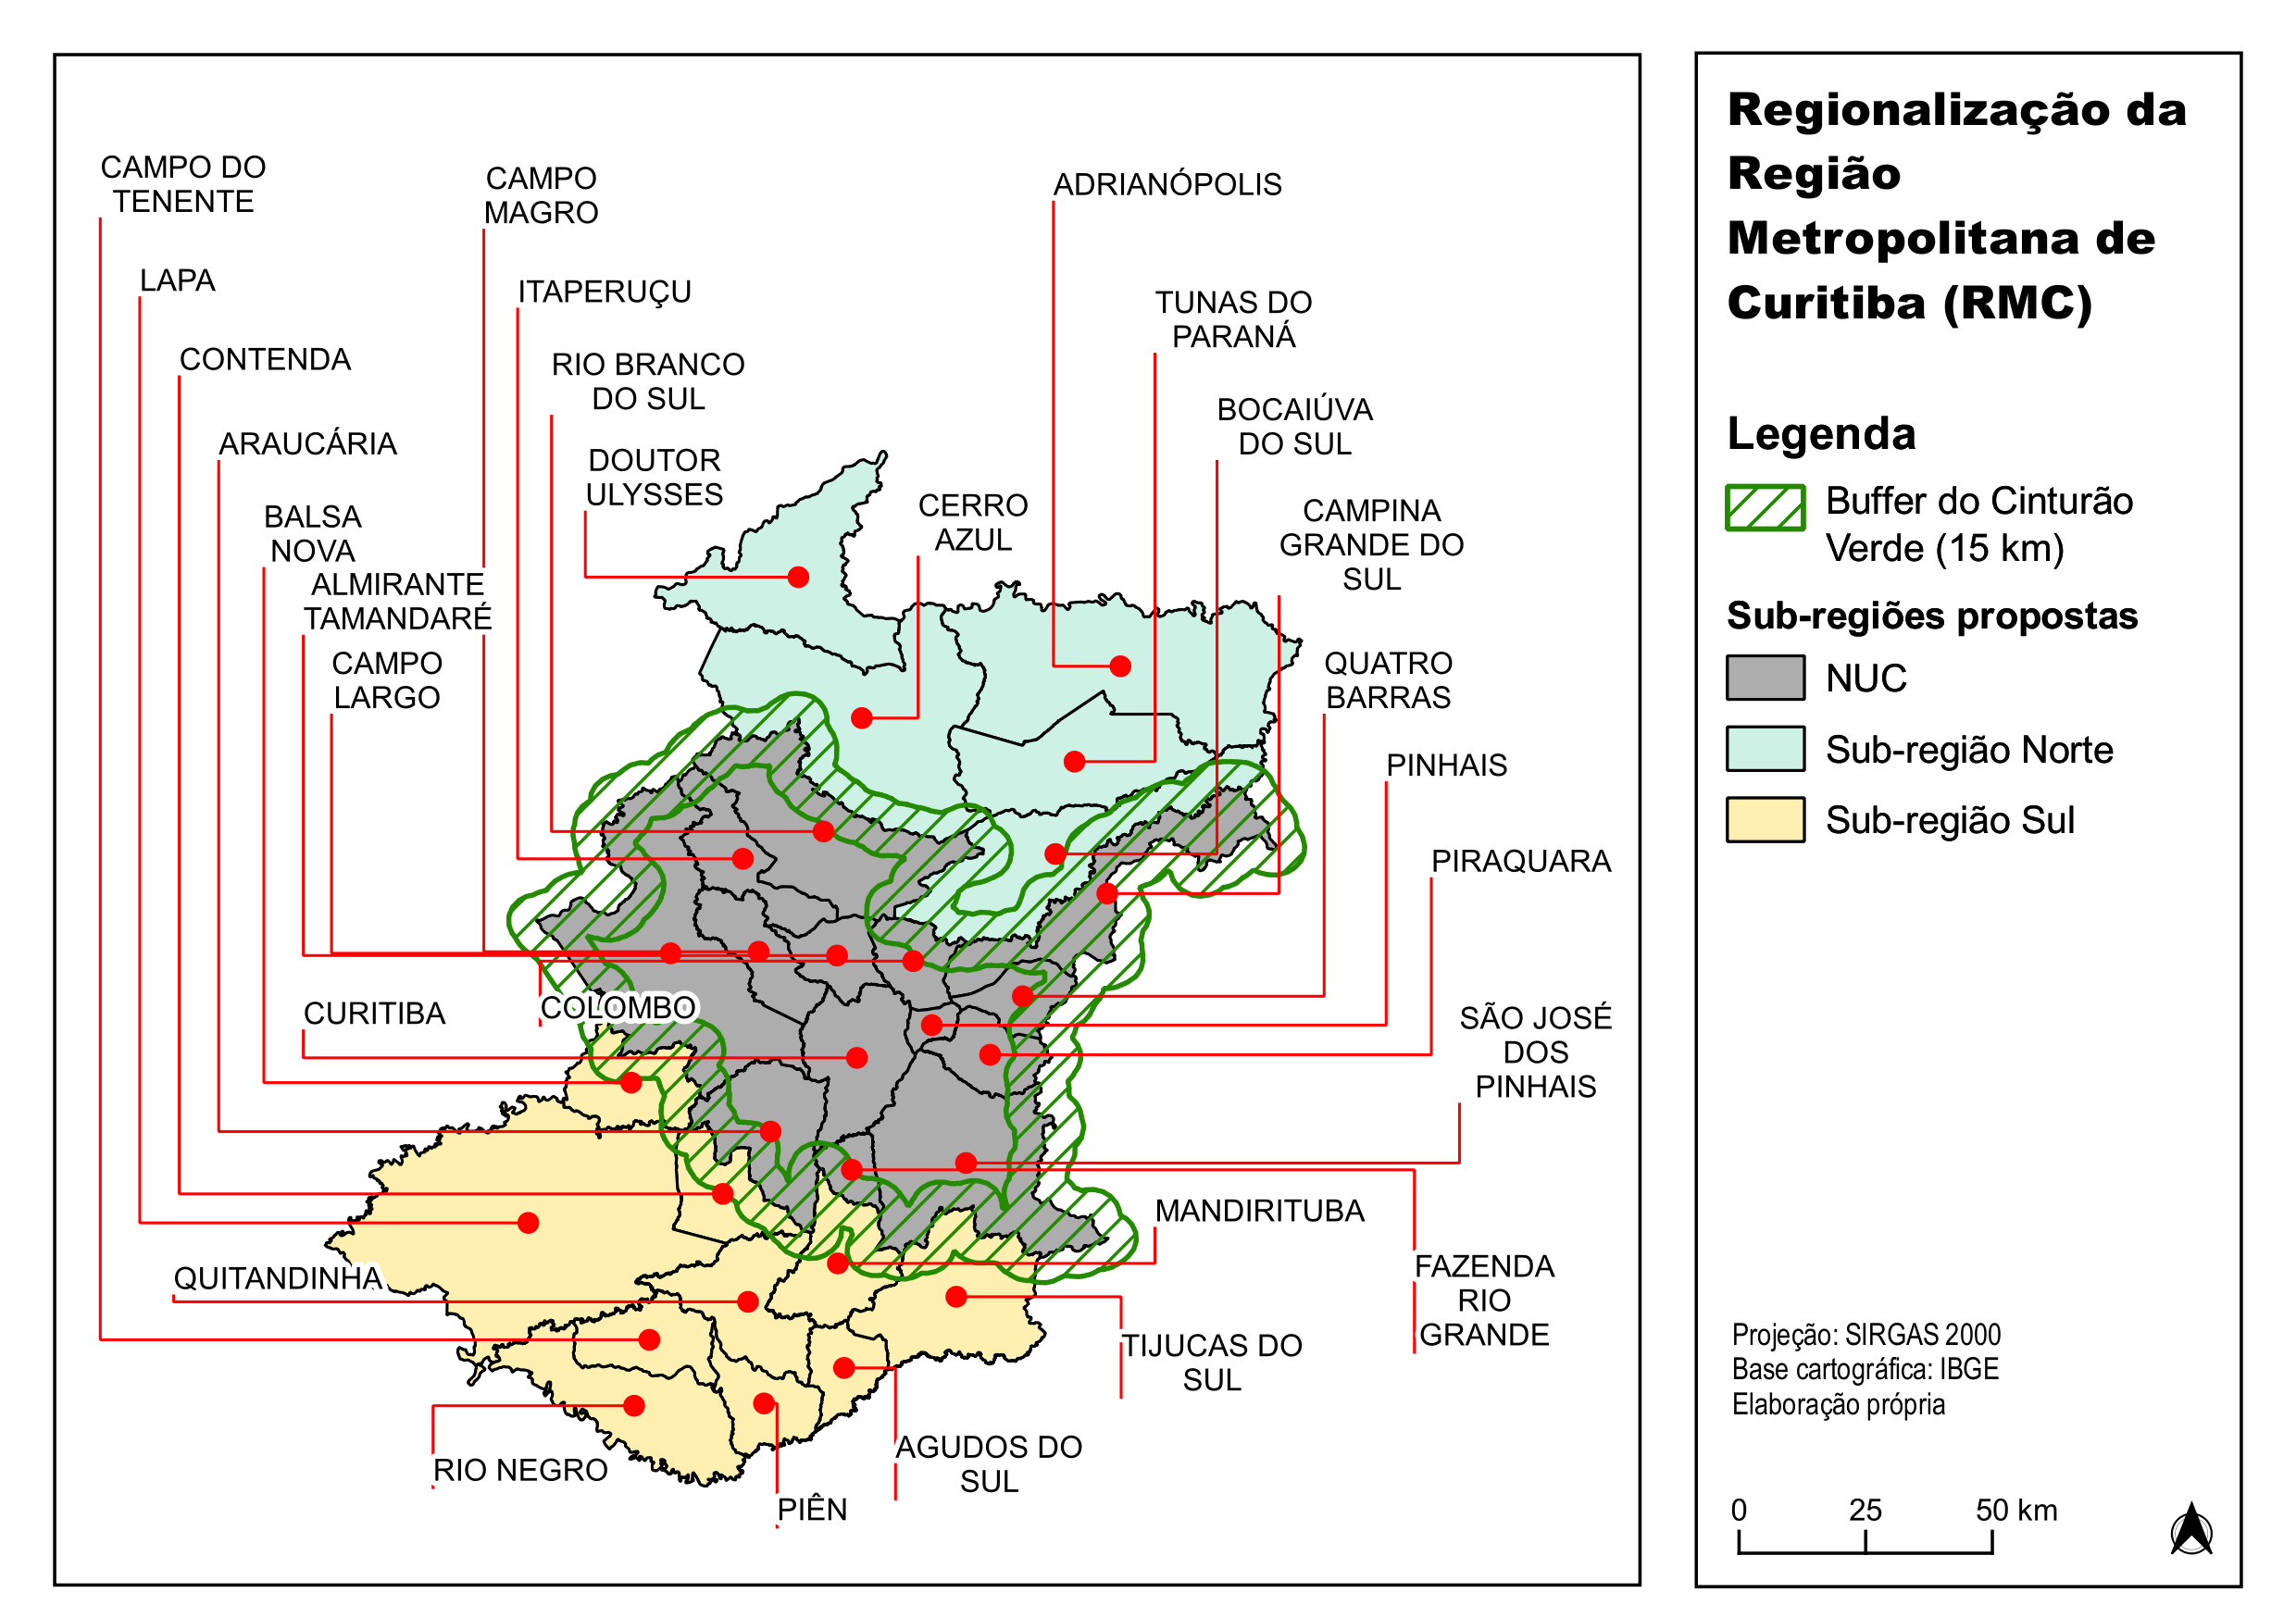
\includegraphics[width=1\linewidth]{../gis/produtos/RMC_subregioes_lei}
	\end{figure}

\end{document}